%%%%%%%%%%%%%%%%%%%%%%%%%%%%%%%%%%%%%%%%%%%%%%%%%%%%
%%          Thai Book Template                    %%
%%                      Anirach Mingkhwan         %%
%% INE-FITM-KMUTNB                18 Aug  2024    %% 
%%%%%%%%%%%%%%%%%%%%%%%%%%%%%%%%%%%%%%%%%%%%%%%%%%%%
% !TEX program = xelatex
\documentclass[11pt,a4paper]{book}

%% ---- Utility package for conditional commands ---- %%
\usepackage{etoolbox}

%% ---- Set up paper margin ---- %%
\usepackage[a4paper,top=1in,bottom=1in,left=1in,right=1in]{geometry}

%% ---- Load the glossaries package for glossary support ---- %%
\usepackage[nonumberlist]{glossaries}
\makeglossaries

%% ---- Set up fonts and encoding ---- %%
\usepackage{fontspec}
\usepackage{xunicode}
\usepackage{xltxtra}

% Enable line breaks for Thai text
\XeTeXlinebreaklocale "th"
\XeTeXlinebreakskip = 0pt plus 2pt minus 1pt

% Set up Thai fonts
\setmainfont[%
    ItalicFont={Laksaman-Italic.otf},%
    BoldFont={Laksaman-Bold.otf},%
    BoldItalicFont={Laksaman-BoldItalic.otf},%
    Script=Thai,%
    Scale=MatchLowercase,%
    WordSpace=1.25,%
    Mapping=tex-text,%
]{Laksaman.otf}

%% ---- Load line spacing package ---- %%
\usepackage{setspace}

% Define a new command for hair space
\newrobustcmd{\hrsp}{\ifmmode\mskip1mu\else\kern0.0625em\fi}

%% ---- Set up hyperlinks and colors ---- %%
\usepackage{xcolor}
\usepackage[unicode=true]{hyperref}
\hypersetup{%
    colorlinks,%
    linkcolor={red!50!black},%
    citecolor={blue!50!black},%
    urlcolor={blue!80!black},%
}
\renewcommand\UrlFont{\normalfont}

%% ---- Load tcolorbox for enhanced code listings ---- %%
\usepackage{tcolorbox}
\tcbuselibrary{listingsutf8} % Support for UTF-8 encoding in listings

%% ---- Load booktabs and caption packages for tables ---- %%
\usepackage{booktabs}
\usepackage{caption}

%% ---- Bibliography Setup with biber backend ---- %%
\usepackage[backend=biber, sorting=none]{biblatex}
\addbibresource{author/bibliography.bib} % Reference the bibliography file

%% ---- Indexing package for creating an index ---- %%
\usepackage{makeidx}
\makeindex

%% ---- Float Package for enforcing specific float positions ---- %%
\usepackage{float}

%% ---- Customizing LaTeX elements to Thai language ---- %%
\renewcommand{\chaptername}{บทที่}  % Change "Chapter" to "บทที่"
\renewcommand{\contentsname}{สารบัญ}  % Change "Contents" to "สารบัญ"
\renewcommand{\indexname}{ดัชนี}      % Change "Index" to "ดัชนี"
\renewcommand{\figurename}{ภาพที่}    % Change "Figure" to "ภาพที่"

% Customizing table caption to Thai
\captionsetup[table]{name=ตาราง}

%% ---- Page Style Setup ---- %%
\usepackage{fancyhdr}
\usepackage{emptypage} % Suppress headers and footers on blank pages

% Set up header height and adjust top margin
\setlength{\headheight}{15.07054pt} % Adjusting the header height
\addtolength{\topmargin}{-3.07054pt} % Compensate for the increased header height

% Set up page style with fancyhdr
\pagestyle{fancy}
\fancyhf{} % Clear all header and footer fields

% Define headers
\fancyhead[LE]{\leftmark}  % "บทที่ X - Chapter Title" on the left side of even pages
\fancyhead[RO]{\rightmark} % Section name on the right side of odd pages

% Define footer
\fancyfoot[C]{\thepage} % Page number at the center of the footer
\renewcommand{\headrulewidth}{0.4pt} % Header line width
\renewcommand{\footrulewidth}{0pt}   % No footer line

%% ---- Documents start here ---- %%
\begin{document}

% ---- Cover page ---- %
\begin{titlepage}
    \centering
    \vspace*{3cm}
    {\Huge \textbf{ชื่อหนังสือ......... (ฉบับร่าง-01)}}\\
    \vspace{1cm}
    {\LARGE ชื่อเรื่องย่อย....}\\
    \vfill
    {\Large Anirach Mingkhwan}\\
    {\large INE-FITM-KMUTNB}\\
    \vspace{2cm}
    \large{\today}
\end{titlepage}

% ---- Front matter ---- %
\frontmatter

\chapter*{คำนำ}

หนังสือเล่มนี้มีจุดมุ่งหมายเพื่อ.......

\begin{flushright}
\textbf{Name Sirname} \\
\textit{Organization} \\
\textit{Date}
\end{flushright} % Include preface
\chapter*{กิตติกรรมประกาศ}

ข้าพเจ้าขอแสดงความขอบคุณ..........

\begin{flushright}
\textbf{Name Sirname} \\
\textit{Organization} \\
\textit{Date}
\end{flushright}
 % Include acknowledgement

\tableofcontents % Generate table of contents

% ---- Main content ---- %
\mainmatter
%%%%%%% Chapter List
\chapter{ชื่อของบท....}

\section{หัวข้อแรก..........}
เนื้อหาแรก....... \Gls{Sample}

\begin{tcolorbox}[colframe=gray!60, colback=gray!6, title=แนวคิดสำคัญ:]
% This part is outside listing so that it won't have line numbers
\begin{itemize}
\item{ {\bf การกำหนดตัวแปร:} การกำหนดค่าให้กับตัวแปร.}
\item{ {\bf การตั้งชื่อตัวแปร:} การกำหนดชือที่เหมาะสมสำหรับตัวแปรตามรูปแบบและแนวทางที่กำหนด.}
\end{itemize}
\end{tcolorbox}


\subsection{หัวข้อย่อยที่ 1 .....ของหัวข้อแรก}
เนื้อหาย่อยของหัวข้อแรก  JavaScript \index{JavaScript}  is nested \index{JavaScript!nested}... .\textcite{flanagan2016javascript}

\subsection{หัวข้อย่อยที่ 2 .....ของหัวข้อแรก}
เนื้อหาย่อยของหัวข้อแรก


\section{หัวข้อที่ 2 ..........}
เนื้อหาแรก.......

\subsection{หัวข้อย่อยที่ 1 .....ของหัวข้อที่ 2}
เนื้อหาย่อยของหัวข้อแรก

\subsection{หัวข้อย่อยที่ 2 .....ของหัวข้อที่ 2}
เนื้อหาย่อยของหัวข้อแรก

\begin{table}[H]
\centering
\caption{ตารางแสดงข้อมูลประชากร}
\label{tab:population}
\begin{tabular}{lrr}
\toprule
\textbf{ประเทศ} & \textbf{ประชากร (ล้านคน)} & \textbf{พื้นที่ (ตร.กม.)} \\
\midrule
ประเทศไทย    & 69   & 513,120 \\
ญี่ปุ่น       & 126  & 377,975 \\
จีน           & 1,400 & 9,596,961 \\
อินเดีย       & 1,366 & 3,287,263 \\
สหรัฐอเมริกา  & 331  & 9,525,067 \\
\bottomrule
\end{tabular}
\end{table}

\section{หัวข้อที่ 3 ..........}
เนื้อหาแรก.......

\subsection{หัวข้อย่อยที่ 1 .....ของหัวข้อที่ 3}
เนื้อหาย่อยของหัวข้อแรก

\subsection{หัวข้อย่อยที่ 2 .....ของหัวข้อที่ 3}
เนื้อหาย่อยของหัวข้อแรก % Include chapter 01
\chapter{ชื่อของบท....}

\section{หัวข้อแรก..........}
เนื้อหาแรก....... \Gls{Example}

\subsection{หัวข้อย่อยที่ 1 .....ของหัวข้อแรก}
เนื้อหาย่อยของหัวข้อแรก latex\index{latex} \textcite{haverbeke2018eloquent}

\subsection{หัวข้อย่อยที่ 2 .....ของหัวข้อแรก}
เนื้อหาย่อยของหัวข้อแรก


\section{หัวข้อที่ 2 ..........}
เนื้อหาแรก.......

\subsection{หัวข้อย่อยที่ 1 .....ของหัวข้อที่ 2}
เนื้อหาย่อยของหัวข้อแรก

\subsection{หัวข้อย่อยที่ 2 .....ของหัวข้อที่ 2}
เนื้อหาย่อยของหัวข้อแรก


\begin{figure}
    \centering
    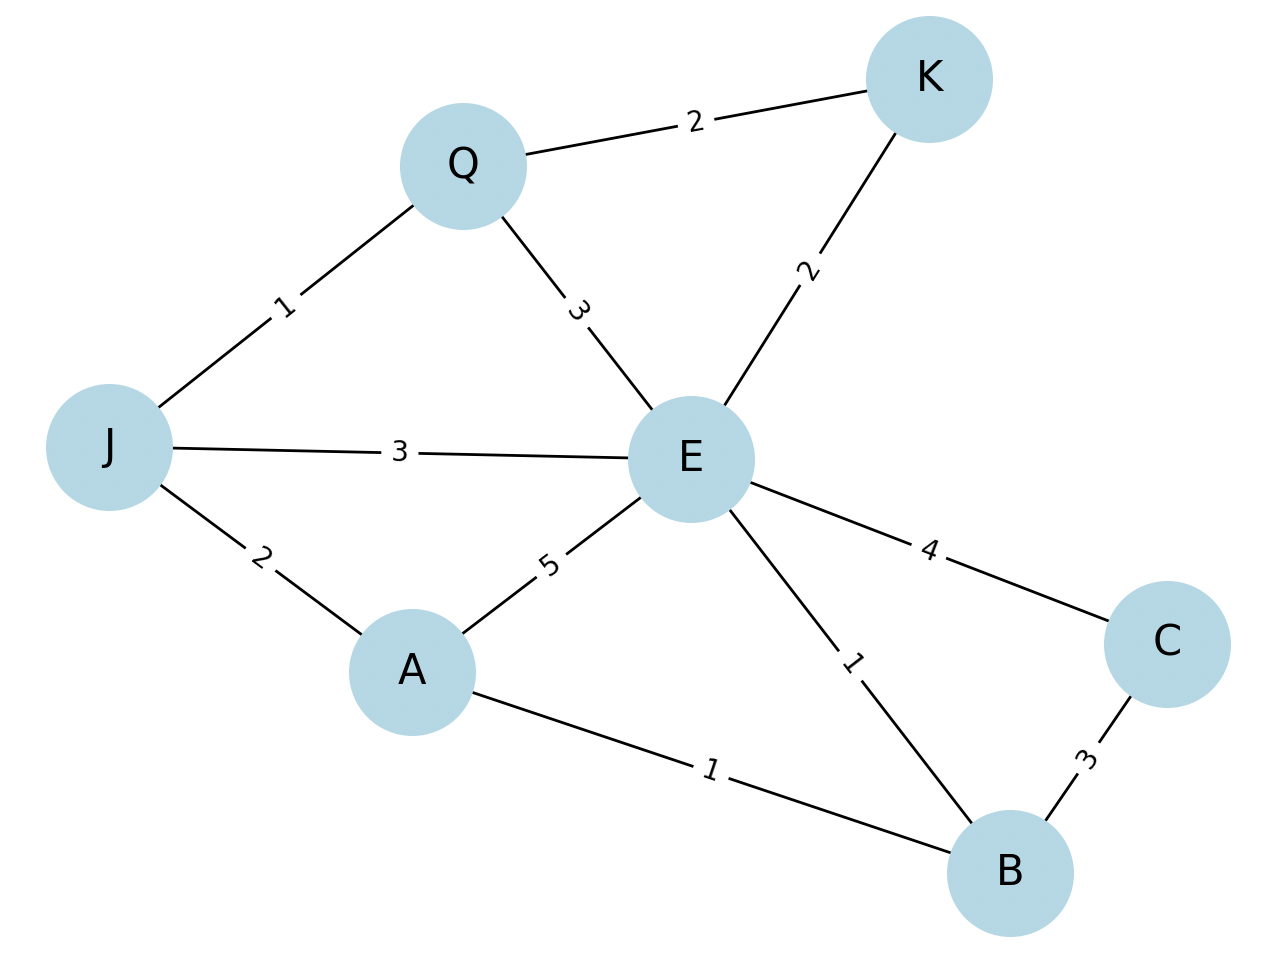
\includegraphics[width=0.5\linewidth]{author//images/graph.png}
    \caption{ใส่ชื่อภาพ}
    \label{fig:enter-label}
\end{figure}
 % Include chapter 02
% Add more chapters as necessary
%%%%%%% End Chapter List

% ---- Back matter ---- %
\backmatter

% Print the bibliography
\clearpage
\addcontentsline{toc}{section}{บรรณานุกรม} % Add Bibliography to TOC
\printbibliography[title=บรรณานุกรม] % Print the bibliography with Thai title

% Print the glossary
\newglossaryentry{DevOps}{
    name=DevOps,
    description={A combination of "Development" and "Operations," representing a set of practices that emphasize collaboration and communication between software developers and IT operations professionals to shorten the software development lifecycle while delivering high-quality software continuously.}
}

\newglossaryentry{Example}{
    name=Example,
    description={This is an example of glossary.}
}
\clearpage
\addcontentsline{toc}{section}{อภิธานศัพท์} % Add Glossary to TOC
\printglossary[title=อภิธานศัพท์] % Print the glossary with Thai title

% Print the index
\clearpage
\addcontentsline{toc}{section}{ดัชนี} % Add Index to TOC
\printindex % Print the index with Thai title

\end{document}
